\chapter{$\Dsplus$ production in p-Pb collisions at $\s$ = 5.02 TeV}
\label{chap:chap6}

In this Chapter the measurements of the ratios of $\Dsplus$-meson yield to that of 
non-strange $\Dplus$ meson are presented as a function of the primary
charged particle multiplicity produced in the p-Pb collision and compared to results from 
pp and Pb-Pb interactions. Primary charged particles are defined as prompt
particles produced in the collisions, including their decay products,
except those from weak decay of strange particles.
In presence of a medium 
composed of deconfined quarks and gluons, a modification of the hadronisation 
mechanisms is expected due to the possible formation of hadrons via
coalescence of charm quarks with other quarks from the 
medium during the deconfined phase or at the phase boundary
~\cite{Greco:2003mm,Greco:2003vf, Andronic:2007zu, He:2012df} in addition to
fragmentation. The enhancement of strange particle production in presence of QGP 
(see Sec.~\ref{subsec:StrangEnhancSPS}) could affect the production of charmed hadrons if 
the dominant mechanism for D-meson formation at low and 
intermediate momenta is in-medium hadronisation of charm quarks 
via recombination with light quarks. In particular, the relative yield of $\Ds$ 
mesons with respect to non-strange charmed mesons at low $\pt$ is 
predicted to be enhanced in nucleus-nucleus collisions as compared to pp 
interactions~\cite{Andronic2003,RafelskiKuznetsova,HeFriesRapp}.
An increase of strangeness production with increasing particle multiplicity was observed 
also in p-Pb and pp collisions~\cite{Abelev:2013haa,Adam:2015vsf,ALICE:2017jyt}. 
If in-medium hadronisation mainly occurs via coalescence at intermediate-low $\pt$, this could result in 
an enhancement of the relative yield of $\Ds$ mesons 
with respect to non-strange charmed mesons in high-multiplicity p-Pb collisions.\\

\section{Event selection}
\label{sec:EvSelpPb}
Events were recorded with a minimum-bias (MB) interaction trigger 
that required coincident signals in both scintillator arrays of the V0 detector.
The V0 timing information was used together with that from the ZDCs for offline rejection 
of events produced by the interaction of the beams with residual gas in the vacuum pipe.
The MB trigger was estimated to be sensitive to about 96.4\% of the p-Pb inelastic cross section.
For the data sample analysed here, the probability of event pile-up in the 
same bunch crossing was below 0.5\% per triggered p-Pb event.
The remaining undetected pile-up (events from different bunch crossings) 
is negligible in the present analysis.
The piled-up events were largely rejected using an algorithm based on the tracklets,
to detect multiple interaction vertices.
Only events with a primary vertex reconstructed within $\pm 10$~cm from the 
centre of the detector along the beam line were considered. 
The number of events passing these selection criteria was about $6\times 10^8$.
The corresponding integrated luminosity is 
$L_{\rm int} =N_{\rm MB}/\sigma_{\rm MB}=292 \pm 11~\mu{\rm b}^{-1}$,
where $\sigma_{\rm MB}=2.09$~b is the MB-trigger (i.e.\ visible) cross section  
measured via a van der Meer scan, with negligible statistical uncertainty 
and a systematic uncertainty of 3.7\%~\cite{Abelev:2014epa}.
During the p-Pb data taking, the beam energies were 4~TeV for 
protons and 1.58~TeV per nucleon for lead nuclei. 
With this beam configuration, the nucleon-nucleon centre-of-mass system 
moves in rapidity by $\Delta y_{\mathrm{cms}}=0.465$ in the direction 
of the proton beam. The D-meson analyses were performed in 
the laboratory-frame interval $|y_{\mathrm{lab}}|<0.5$, 
which leads to a shifted centre-of-mass rapidity coverage 
of $-0.96 < y_{\mathrm{cms}} < 0.04$.\\


During the p-Pb data taking, two different detector clusters were used to collect data, depending on the 
availability of the SDD in the readout. Consequently, the respective reconstructions have different
detector configurations, thus their $\pt$ resolution may differ. It was verified that the 
width and the position of the D-meson signal peak were compatible in the two
reconstruction, as a function of $\pt$.The two samples were hence merged and both
used in the analysis in order to maximise the statistics.

\begin{figure}[h]
\centering
 \includegraphics[width=.6\textwidth]{FigCap6/NtrklVsVxtZ_Data.png}
 \caption{Tracklets distribution as a function of the z-vertex coordinate for the periods 16q and 16t, and for both FAST and CENT reconstructions.}
 \label{fig:NtrklVsZ2D}
\end{figure}


\section{Equalisation of N$_{\rm tracklets}$ distribution as a function of $z_{\rm vtx}$}
\label{sec:zVxtEq}
The ratios of $\Dsplus$ /$\Dplus$ production yields were studied as a 
function the charged-particle multiplicity in different $\pt$ intervals.
The multiplicity estimator used for this analysis was based on the number 
of tracklets reconstructed in the SPD within a 
pseudo-rapidity range of $|\eta| <$ 1. A tracklet in the SPD is obtained by
joining space points on the two SPD layers and it is required to point to 
the reconstructed primary vertex. 
Events that do not have a reconstructed vertex do not pass the selection criteria, hence
do not contribute to the tracklet distribution. 
In Fig.~\ref{fig:NtrklVsZ2D}, the distribution of tracklets ($\Ntrkl$) as a function
of the $z$ coordinate of the vertex ($\zVtx$) is shown.
 The average profiles of the distributions can also be observed superimposed on the plots
 and it reveals a dependence of the average $\averNtrkl$ on $\zVtx$. 
 The trend of $\averNtrkl$ as a function of $\zVtx$ is related to the SPD acceptance.
 The modification of the SPD configuration during the data acquisition 
 modifies also the number of reconstructed tracklets.
 Lower $\averNtrkl$ values towards $\zVtx \sim 10 $ cm are due to the 
 finite acceptance of the SPD layers. 
The distribution of $\Ntrkl$ vs $\zVtx$ needs to be equalised 
in order to define consistently the $\Ntrkl$ intervals in which the analysis is performed.
Otherwise, a given $\Ntrkl$ interval would correspond to different real charged particle
multiplicities, depending on $\zVtx$ or data taking period.
On this purpose, the average profile of $\Ntrkl$ vs $\zVtx$ was analysed on a run-by-run basis 
over the full period, to evaluate the stability of $\averNtrkl$ as a function of $\zVtx$ 
as a function of time. Four bunches of runs were found with 
up to $\sim$10\% difference in the $\averNtrkl$ values at positive values 
of $\zVtx$, as shown in Fig.~\ref{fig:FourBunches} (left).
 The equalisation of $\averNtrkl$ over the $\zVtx$ was applied on an 
 event-by-event basis on each of the four bunches of runs separately.
The $\averNtrkl$ value that was used as the absolute reference multiplicity 
value was defined as the maximum of $\averNtrkl$ distribution as a function of $\zVtx$,
resulting $\Ntrkl =  29.2$. 
The number $N_{\rm raw}$ of reconstructed tracklets in an event
is corrected by using a Poissonian extraction as follows:
\begin{equation} 
\label{eq:NtrklCorr}
N_{\rm corr} = N_{\rm raw} + {\rm Pois}(\Delta N),
\end{equation}
with:
\begin{equation} 
\label{eq:NtrklCorr}
\Delta N = \Big (\frac{N_{\rm ref}}{\langle N(\zVtx) \rangle} -1 \Big ) \cdot N_{\rm raw}.
\end{equation}
 It is advisable that the reference multiplicity value $N_{\rm ref}$ is chosen as the
 maximum value of the $\averNtrkl$ distribution, in order to assure
 that $N_{\rm corr}$ is a Poissonian variable. 
The average $\averNtrkl$ profiles of the four bunches of runs 
after the $\zVtx$ equalisation are shown in the right panel of 
Fig.~\ref{fig:FourBunches}, eventually fitted with a pol1 function in order
to check the flatness of the distribution. 

\begin{figure}[h]
\centering
 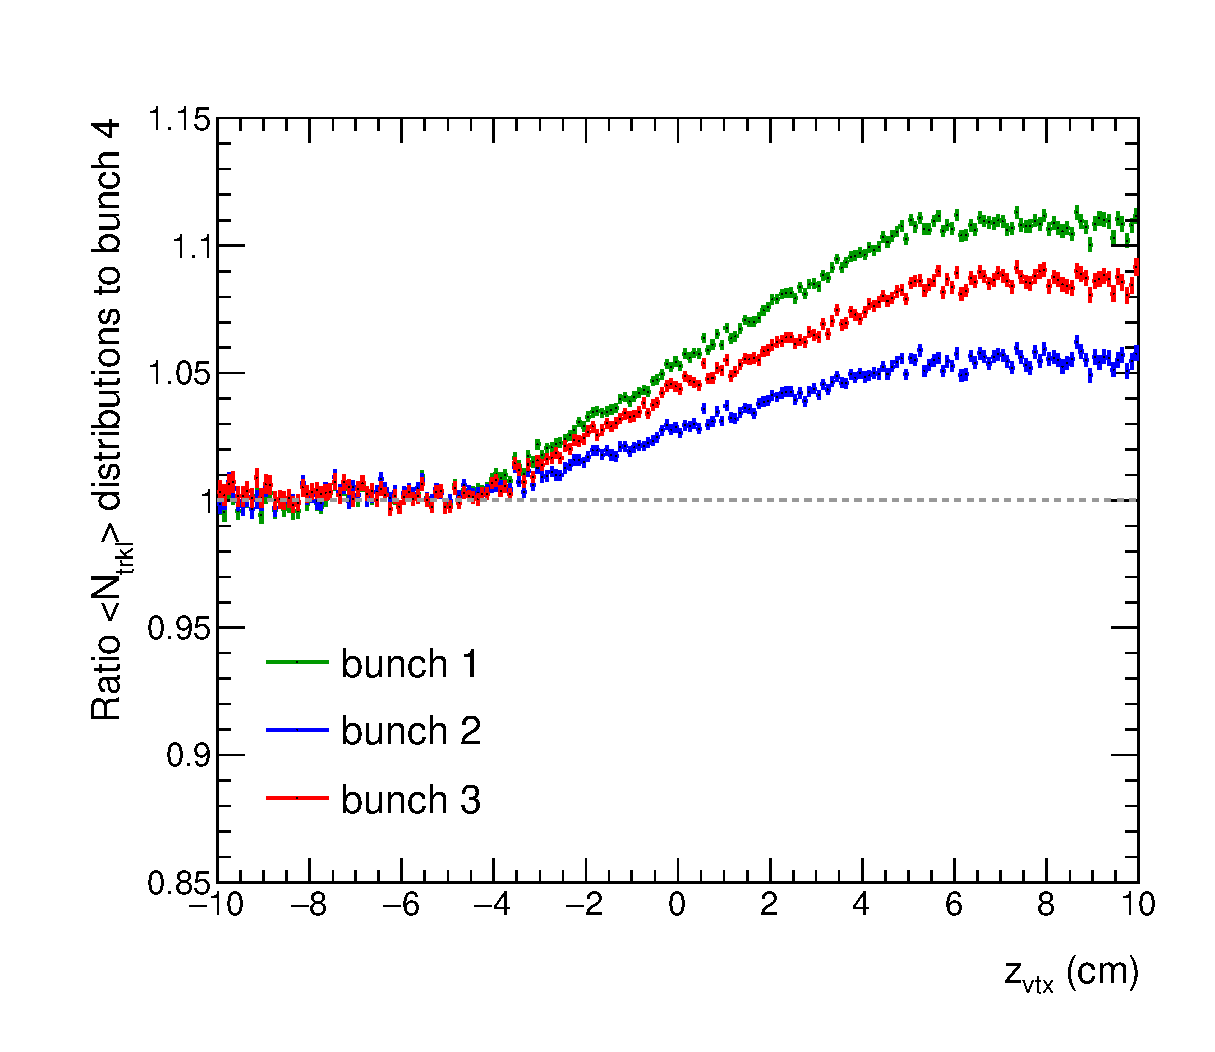
\includegraphics[width=.49\textwidth]{FigCap6/UncorrNtrklProfileDataRatio.eps}
 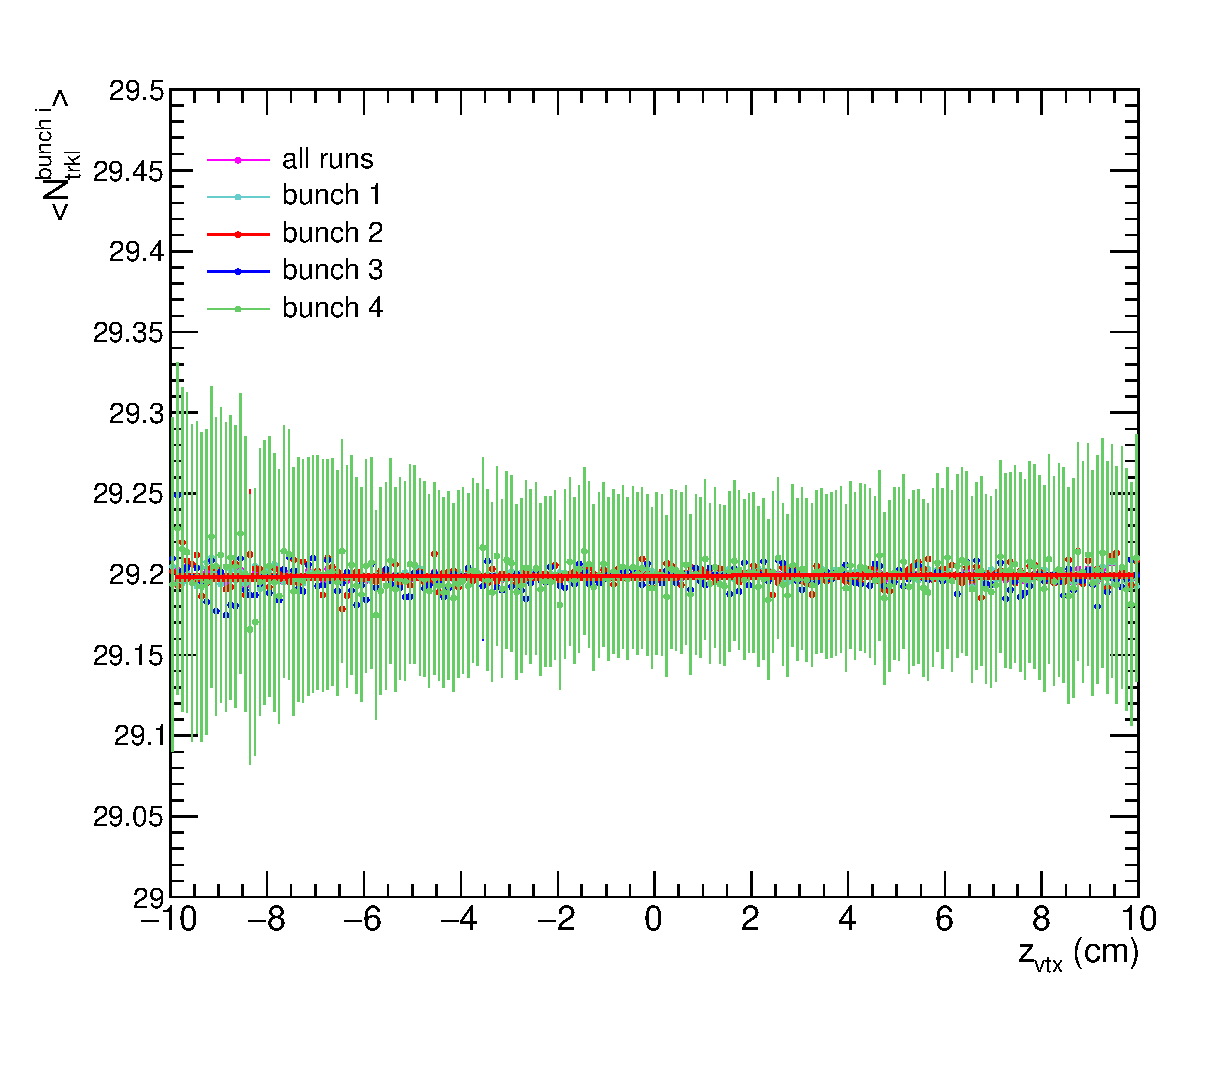
\includegraphics[width=.49\textwidth]{FigCap6/NtrkProfilesDataAfterZVxtEqual.eps}
 \caption{Left: average $\averNtrkl$ distributions as a function of $\zVtx$ for the four bunches of runs in different colours. Right: average $\averNtrkl$ distributions as a function of $\zVtx$ for the four bunches of runs in different colours, after the equalisation over $\zVtx$.}
 \label{fig:FourBunches}
\end{figure}

\section {Raw-yield extraction}
\label{sec:Rawyields_vs_mult}
The $\Ds$ signal was extracted in five $\pt$ intervals from 2 to 16 $\Gevc$, 
in three different classes of $N_{\rm trkl}$: $[1,40)$, $[40,70)$, $[70,200]$ tracklets.
The intervals were chosen in order to have sufficient statistics for the $\Ds$-meson yield extraction.
They contain, in the order, 27.5\%, 40.5\% and 30\% of total events.
The same topological selections were used in the three multiplicity class in each $\pt$
interval and they were tuned to have good statistical significance of the extracted yields.
They are summarized in Tab.~\ref{tab:cutsDsVsNtrkl}.
\begin{table}[h!]
\centering
\begin{tabular}{|l|c|c|c|c|c|}
\hline
$\Ds$ topological selections & \multicolumn{5}{c|}{pt interval (GeV/$c$)}\\
\cline{2-6}
  & 2--4  & 4--6 & 6--8 & 8--12 & 12--16\\
\hline
Decay length ($\mum$)        & $>$300 & $>$350 & $>$350 & $>$400& $>$400\\
Decay length XY ($\mum$)     & $>$0 & $>$200 & $>$200 & $>$200 & $>$200\\
Norm Decay length XY          & $>$2.0& $>$0.0 & $>$2.0 & $>$2.0 & $>$2.0\\
Cosine pointing              & $>$0.94 & $>$0.95 & $>$0.95 & $>$0.97 & $>$0.97\\
$\sigma_{vertex}$  (cm)          & $<$0.02 & $<$0.03 & $<$0.03 & $<$0.06 & $<$0.06\\
$\Delta M$ (MeV/$c^{2}$) & $<$8.0 & $<$10.0 & $<$4.5 & $<$9.0 & $<$9.0\\
$\cos \theta^*(\pi)$    & $<$1.0 & $<$1.0 & $<$1.0 & $<$0.95 & $<$0.95\\
$|\cos^3 \theta^\prime({\rm K})|$        & $>$0.10 & $>$0.05 & $>$0.05 & $>$0.05 & $>$0.05\\
Norm. IP residual  & $<$2.5 & $<$2.0 & $<$2.0 & $<$2.0  & $<$2.0 \\
\hline
\end{tabular}
\caption{Topological selections used for the $\Ds$ meson in the five transverse momentum intervals consideredfor the three $N_{\rm trkl}$ classes.}
\label{tab:cutsDsVsNtrkl}
\end{table}
Fig.~\ref{fig:DsInvMassVsNtrkl_1},~\ref{fig:DsInvMassVsNtrkl_2} and~\ref{fig:DsInvMassVsNtrkl_3} 
show the invariant-mass fits performed in the five $\pt$ intervals, for the three 
multiplicity classes. The second peak on the left of $\Ds$ signal, around 1.88 MeV/$c^2$,
corresponds to $\Dplus$ decay contribution in the same channel considered of $\Ds$.
\begin{figure}[htpb]
\centering
 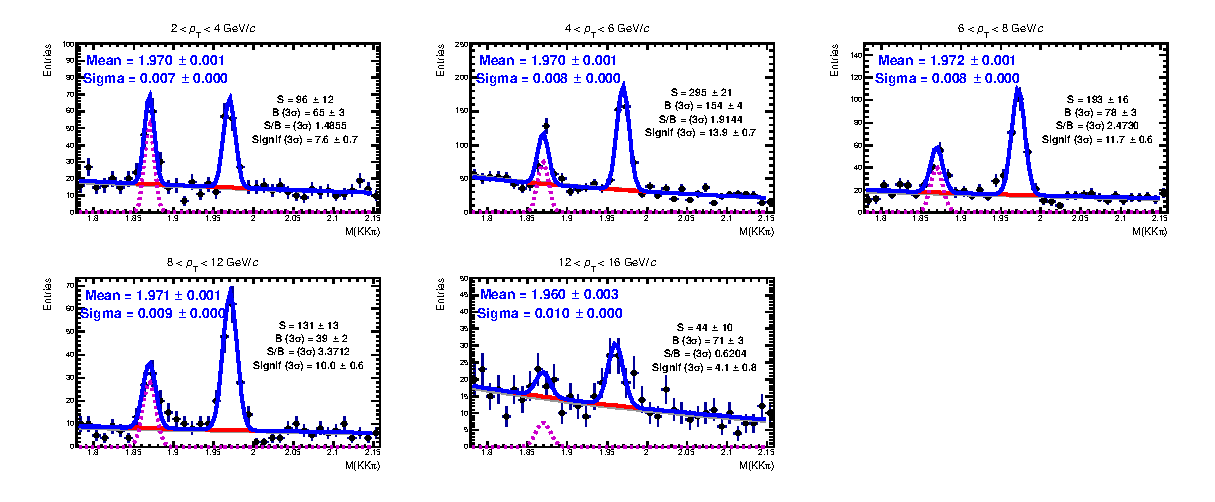
\includegraphics[width=1\textwidth]{FigCap6/DsMass_140Trkl.eps}
  \caption{$\Dsplus$ invariant-mass spectra, from 2 to 16 $\Gevc$, in the $1 \leq N_{\rm trkl} < 40$ interval.}
 \label{fig:DsInvMassVsNtrkl_1}
\end{figure}
\begin{figure}[htpb]
\centering
 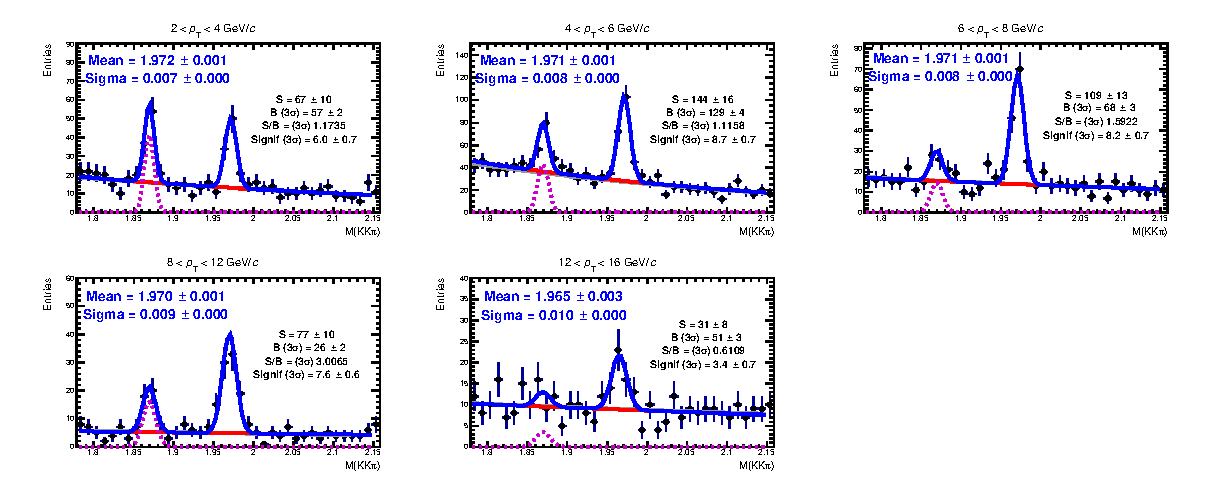
\includegraphics[width=1\textwidth]{FigCap6/DsMass_4070Trkl.eps}
  \caption{$\Dsplus$ invariant-mass spectra, from 2 to 16 $\Gevc$, in the $40 \leq N_{\rm trkl} < 70$ interval.}
 \label{fig:DsInvMassVsNtrkl_2}
\end{figure}
\begin{figure}[htpb]
\centering
 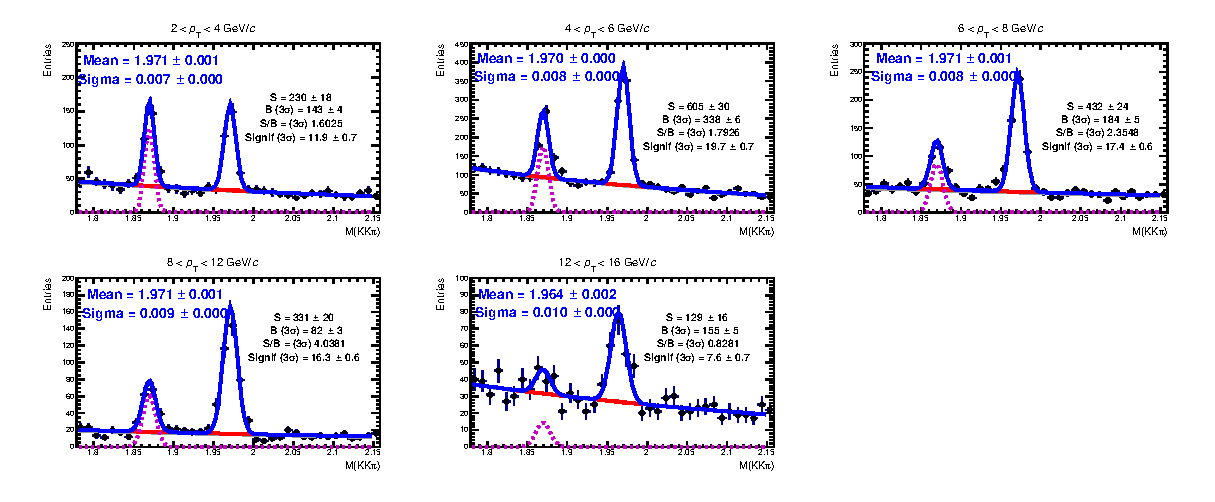
\includegraphics[width=1\textwidth]{FigCap6/DsMass_70200Trkl.eps}
  \caption{$\Dsplus$ invariant-mass spectra, from 2 to 16 $\Gevc$, in the $70 \leq N_{\rm trkl} \leq 200$ interval.}
 \label{fig:DsInvMassVsNtrkl_3}
\end{figure}
To avoid fluctuations, the $\Ds$ peak widths were fixed to the values obtained from the 
minimum-bias simulation (which were verified to be compatible to the values
from minimum-bias fit in data). In Fig.~\ref{fig:DsFitParamsVsNtrkl} 
the comparison of the Gaussian mean and width 
in data and minimum-bias MC is shown, as an example for the interval $40 \leq N_{\rm trkl} < 70$. 

\begin{figure}[htpb]
\centering
 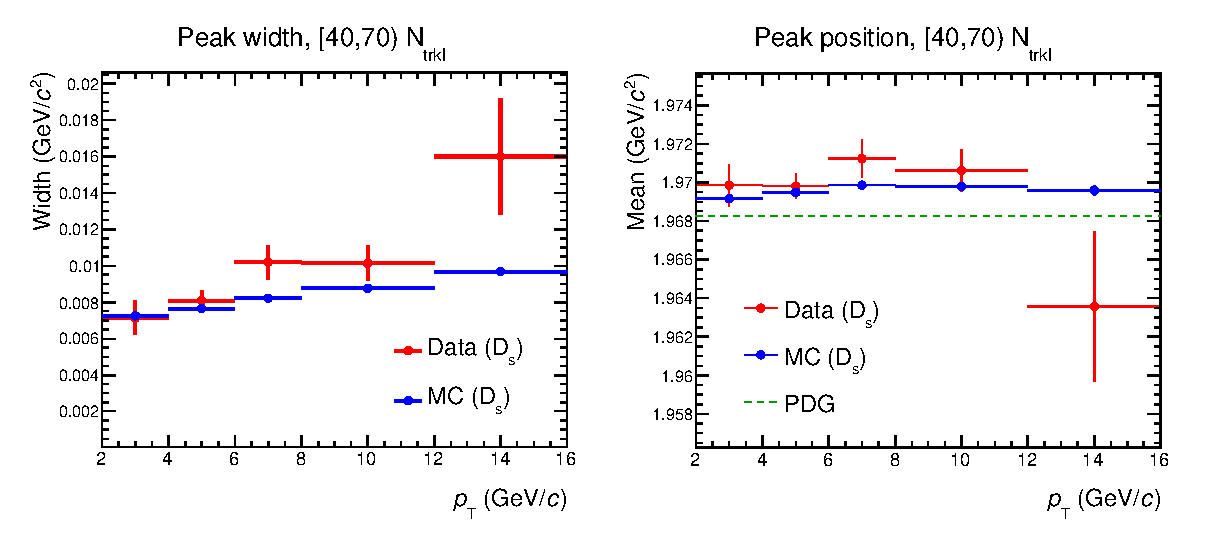
\includegraphics[width=1\textwidth]{FigCap6/DsMeanSigma_DataMC_4070_Ntrkl.eps}
  \caption{$\Ds$ (and $\Dplus$ in the same $\Ds$ decay channel) peak width (left) and mean (right) obtained in the $N_{\rm trkl}$ intervals compared to the values from the data in the interval $40 \leq N_{\rm trkl} < 70$ and the minimum-bias MC simulation.}
 \label{fig:DsFitParamsVsNtrkl}
\end{figure}

\section{Corrections}
\label{sec:Corrections}
The $\Dsplus$/$\Dplus$ ratios in the multiplicity class $i$ were calculated
as:
\begin{equation} 
\label{eq:NtrklCorr}
 \frac{({\rm d}^2N_{\Ds}/{\rm d}\pt {\rm d}y)}{({\rm d}^2N_{\Dplus}/{\rm d}\pt {\rm d}y)} \Big |_i = \frac{Y^i_{\Ds}  f^i_{\rm prompt, \Ds} / ({\rm Acc} \times \epsilon)^i_{\rm prompt \Ds}}{Y^i_{\Dplus}  f^i_{\rm prompt, \Dplus} / ({\rm Acc} \times \epsilon)^i_{\rm prompt \Dplus}} \cdot \frac{\rm BR(\DstoKKpi)}{\rm BR(\DplustoKpipi)},
\end{equation}
where $Y$ is the extracted yield, which is corrected for the prompt fraction
$f_{\rm prompt}$, for the acceptance-times-efficiency term $({\rm Acc} \times \epsilon)$ and for
the branching ratio BR of the decay channel.\\



The acceptance-times-efficiency term was obtained via Monte Carlo simulations
using PYTHIA v6~\cite{Sjostrand:2006za} with Perugia-2011 tuning as event generator and 
particles were transported through the detectors using GEANT3 package~\cite{Brun:1994aa}.
A $N_{coll}$ value is extracted for each PYTHIA event via a minimum-bias 
distribution obtained starting from a Glauber MC simulation. If the 
extracted number of binary collisions is larger than 1, a HIJING~\cite{Wang:1991hta} p-Pb 
event is added as the underlying event. 
Fig.~\ref{fig:NtrklDataMC} shows the distributions of $\Ntrkl$ in data and simulation.
The events selected to fill the distributions were required to have at least a $\Dzero$-meson candidate 
with the invariant mass compatible within 3$\sigma$ to the PDG $\Dzero$ mass.
The real distribution was already corrected for the $\zVtx$ equalisation. 
To not introduce differences at the level of the multiplicity selection between data and MC, 
the distribution in the minimum-bias simulation needs to be corrected
with data-driven weights. It can also be noticed that
the simulated $\Ntrkl$ distribution reaches
lower $\Ntrkl$ values with respect to data. It was verified 
that the selection efficiency of $\Ds$ meson is not dependent on
the tracklet multiplicity above 20 tracklets per event, so the different
maximum $\Ntrkl$ values in data and MC does not constitute an issue.
The correction factor for the MC distribution was calculated independently for each of the 
four groups of runs described in Sec.~\ref{sec:zVxtEq}. Fig.~\ref{fig:RatioNtrklMC}
shows the ratio of the $\Ntrkl$ distributions of each of the four bunches
of runs to the distribution of the minimum-bias sample, to 
better clarify the necessity of four distinct corrections on the simulation.
The weights obtained for the selection efficiencies are shown in Fig.~\ref{fig:MCweights}.
The resulting acceptance-times-efficiency terms are presented in 
Fig.~\ref{fig:DsEffVsMult} as a function of $\Ntrkl$, for the five $\pt$ intervals
in different colours. As shown in this figure, the efficiency is almost flat 
as a function of the event multiplicity, and the largest difference is 
observed between the first $\Ntrkl$ interval and the other two, as expected.


\begin{figure}[h]
\centering
 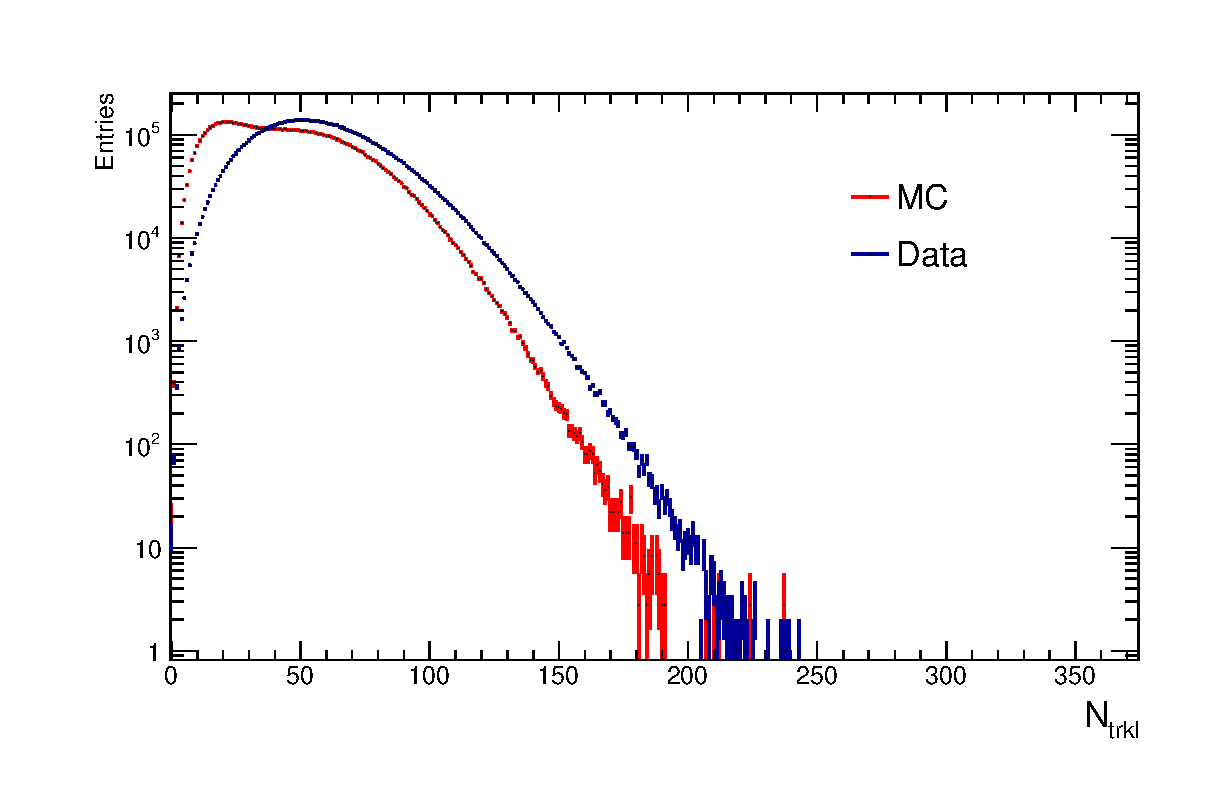
\includegraphics[width=.5\textwidth]{FigCap6/NtrkDistrDDataMC.eps}
 \caption{Tracklets distribution in data and in MC in different colours.}
 \label{fig:NtrklDataMC}
\end{figure}

\begin{figure}[h]
\centering
 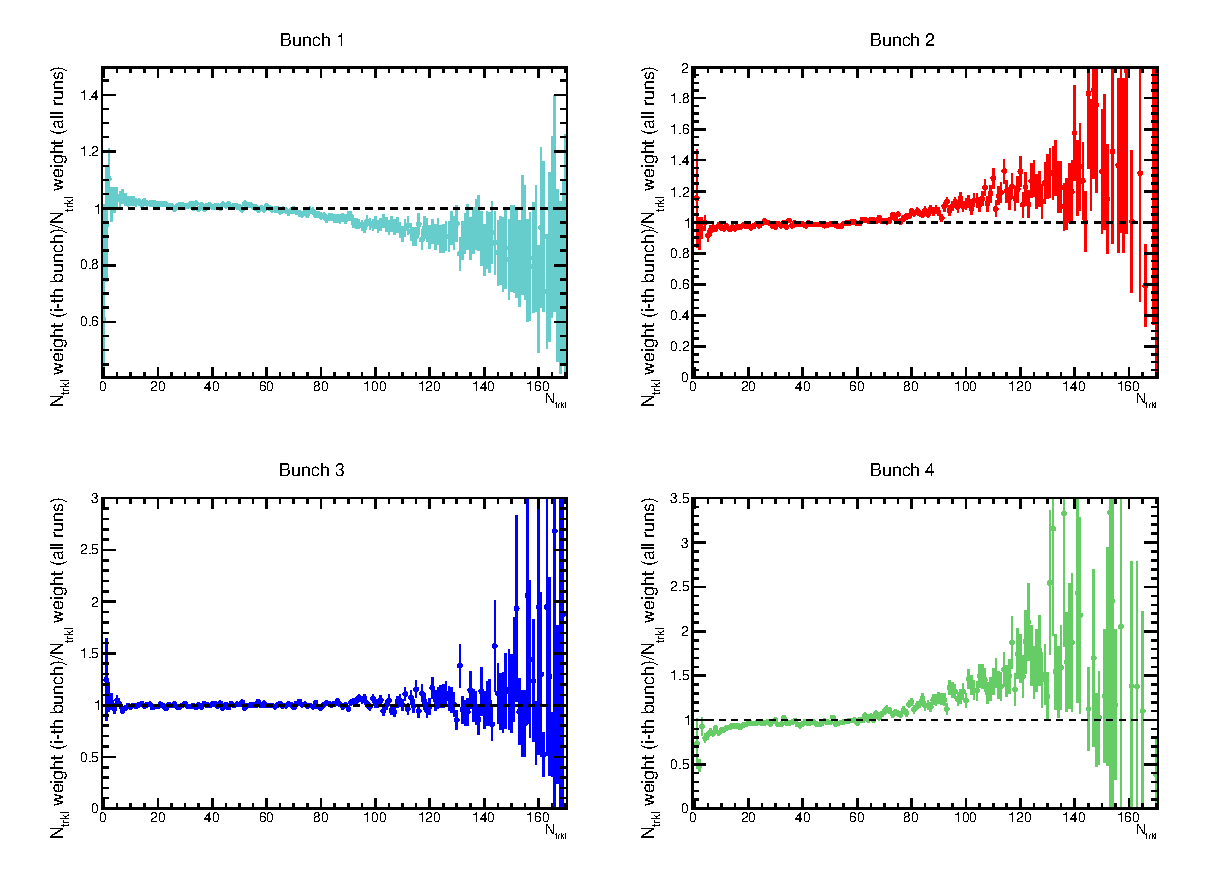
\includegraphics[width=.9\textwidth]{FigCap6/NtrkDistrMC_17d2a_EvWithD_zVxtUnCorr_896_897.eps}
 \caption{Ratio of the $\Ntrkl$ distribution for the MC in each of the four bunches of runs over the distribution obtained with the full statistics.}
 \label{fig:RatioNtrklMC}
\end{figure}

\begin{figure}[h]
\centering
 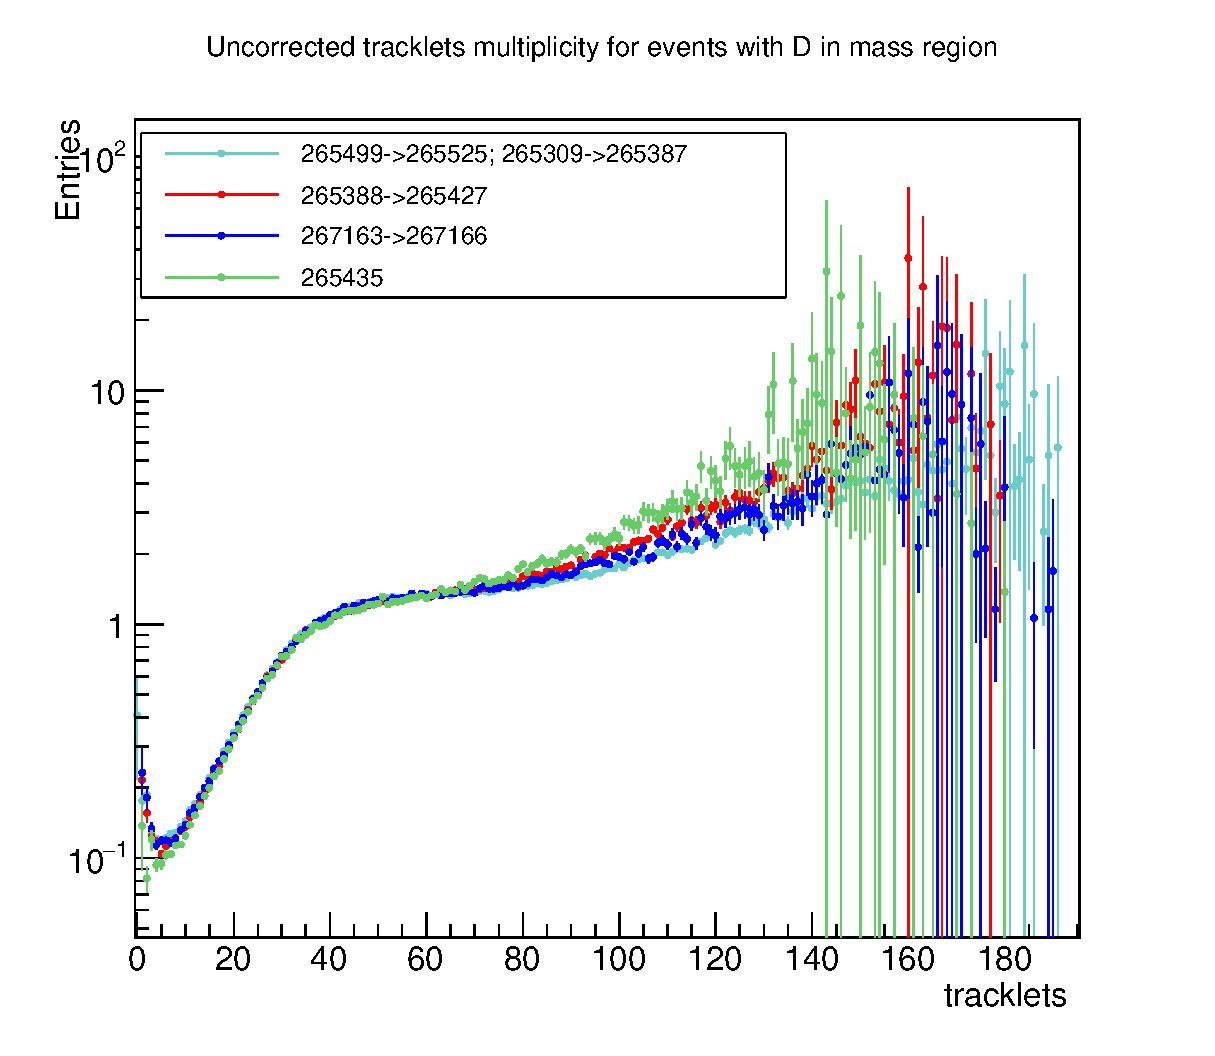
\includegraphics[width=.55\textwidth]{FigCap6/NtrklWeights4Bunches.eps}
 \caption{$\Ntrkl$-weight distributions for the MC in each of the four bunches of runs in different colours.}
 \label{fig:MCweights}
\end{figure}

\begin{figure}[h]
\centering
 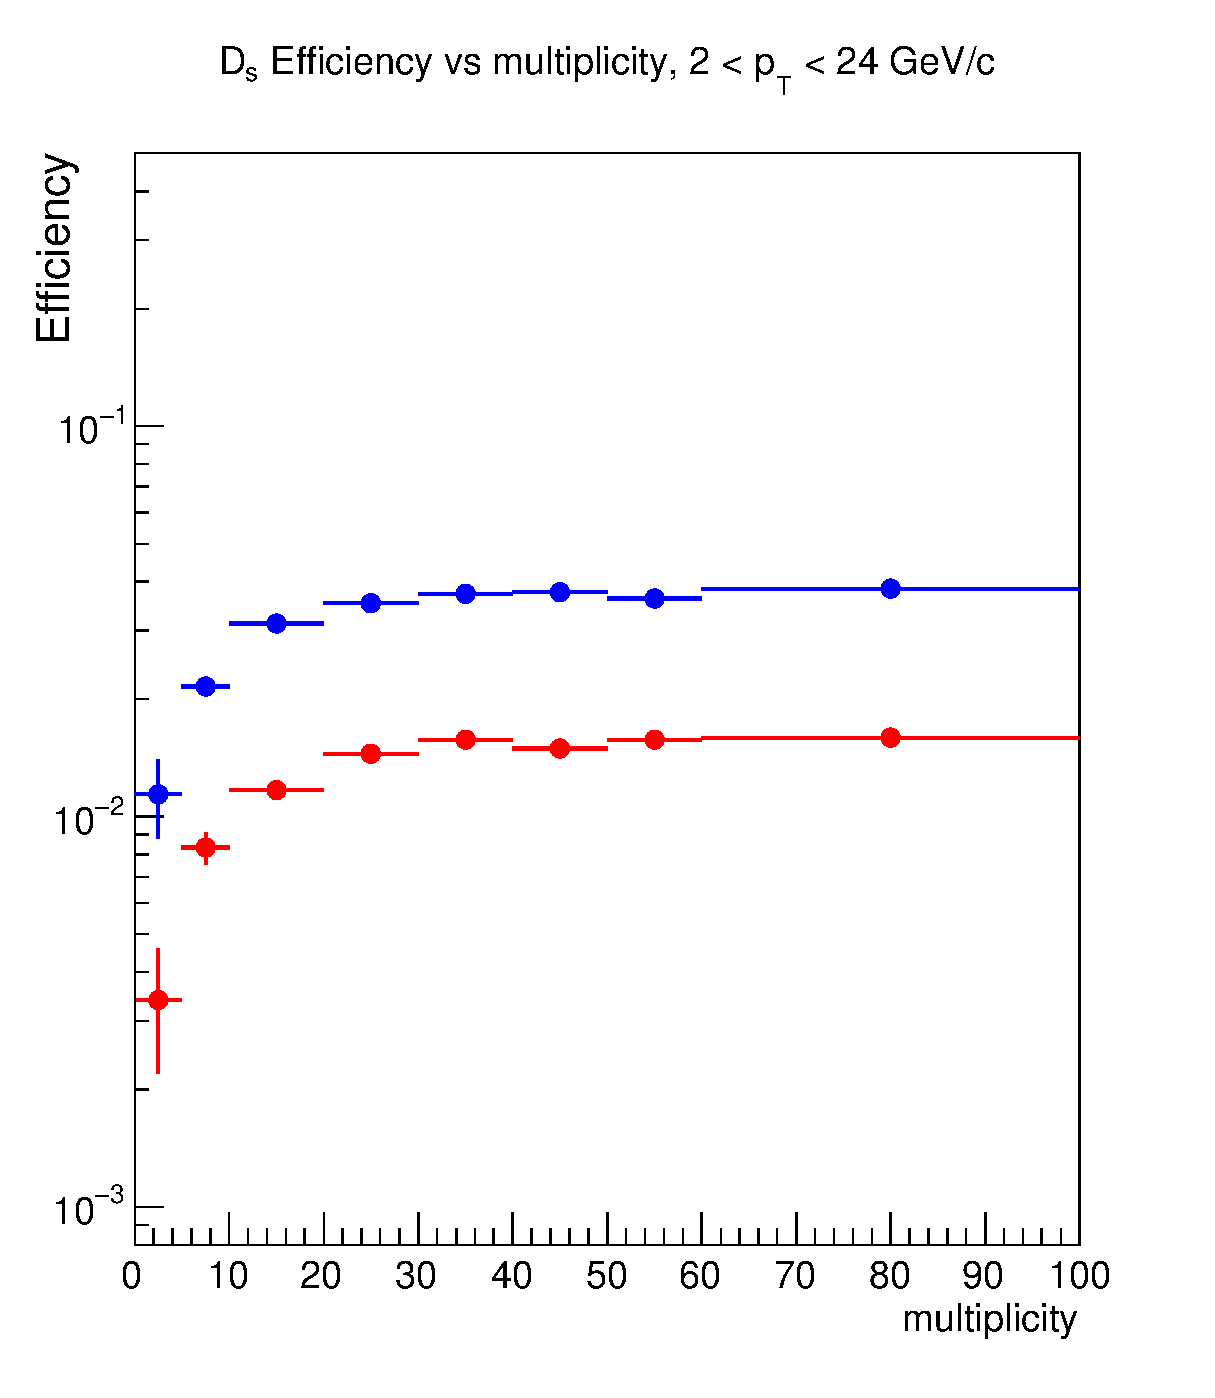
\includegraphics[width=.45\textwidth]{FigCap6/DsEffvsMult_pPb2016.eps}
 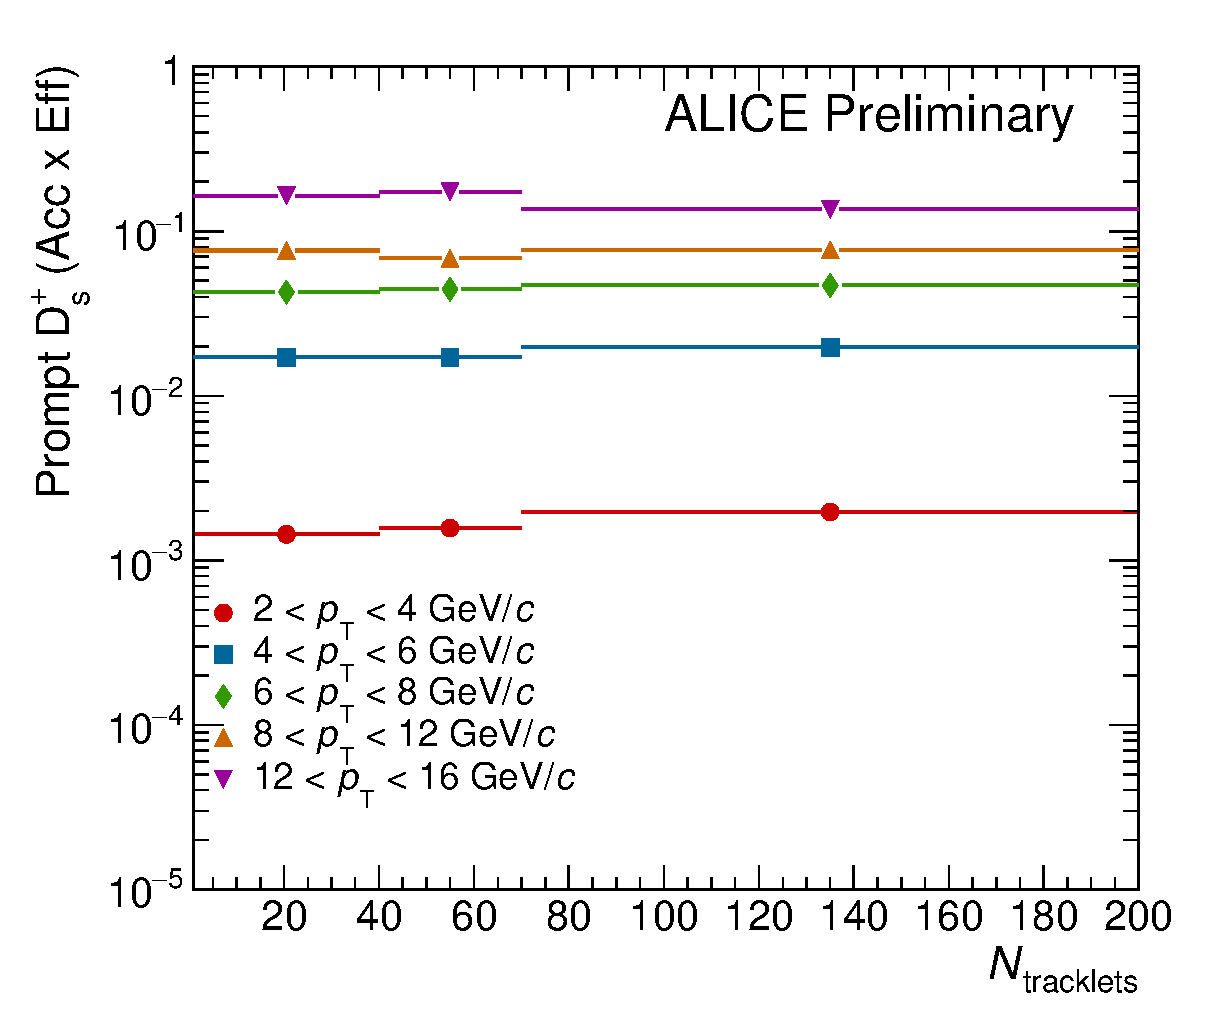
\includegraphics[width=.45\textwidth]{FigCap6/PromptDsEfficiency_times_Acceptance_VsNtrkl.eps}
 \caption{$\Ds$ efficiency as a function of the tracklet multiplicity, $\pt$-integrated between 2 and 24 $\Gevc$, in red for prompt and in blue for the feed-down.}
 \label{fig:DsEffVsMult}
\end{figure}



\subsection {Feed-down subtraction}
For the feed-down subtraction, the FONLL-based method 
described in Eq.~\ref{eq:fprAA} was used. It was 
assumed that the fraction of prompt $\Ds$ does not depend on the 
multiplicity and therefore the prompt fraction computed considering 
the minimum-bias sample (Fig~\ref{fig:DsfPrompt}) was used for all the $\Ntrkl$ classes. 
This hypothesis also holds for $\Dplus$ meson and is supported 
by the results obtained for the D-meson $\QpPb$ analysis on the same data sample~\cite{ALICEPAS2017008}, 
were the fraction of prompt D mesons in the two centrality classes used (0-10\% and 60-100\%
percentiles of ZNA) and in the minimum-bias sample are compatible. 
In Eq.~\ref{eq:fprAA}, a hypothesis on $\RAA^{\rm feed-down}$
is applied to account for different modification of beauty and charm 
production in Pb-Pb collisions. In a similar way, for the calculation of $f_{\rm prompt}$ in 
the minimum-bias p-Pb sample, the assumption of $R_{\rm pPb}^{\rm feed-down} = R_{\rm pPb}^{\rm prompt}$ 
is done, for both $\Ds$ and $\Dplus$ mesons.
%This hypothesis was then varied between 
%$0.9 < R_{\rm pPb}^{\rm feed-down} = R_{\rm pPb}^{\rm prompt} <1.3$ 
%to estimate the systematic uncertainty, as will be described in more details in the dedicated section. 

\begin{figure}[htpb]
\centering
 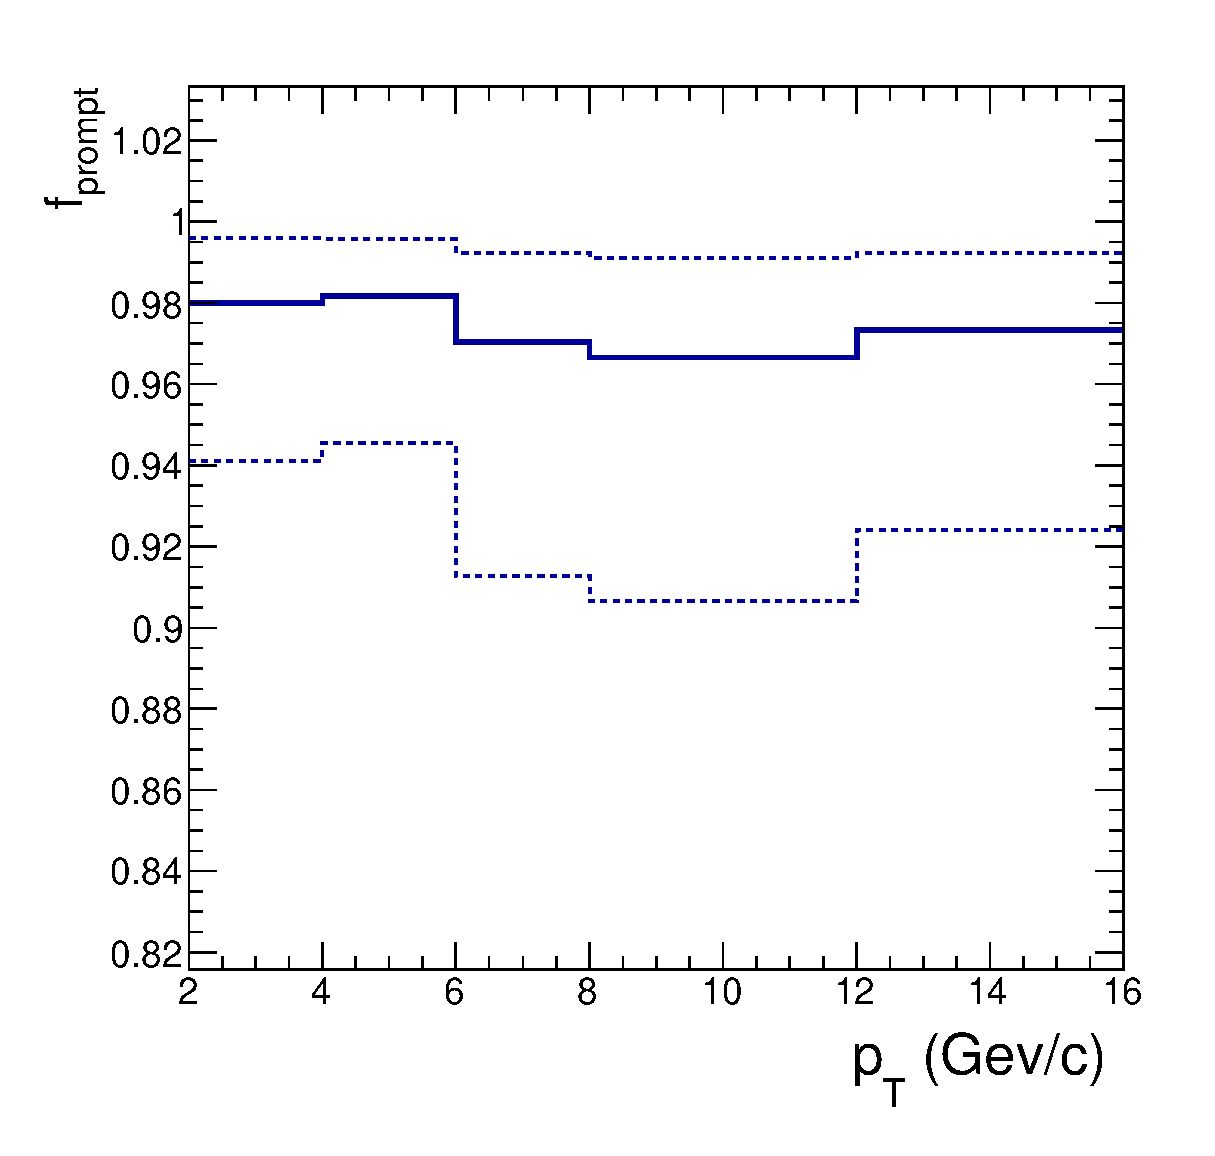
\includegraphics[width=.7\textwidth]{FigCap6/DsFPrompt.eps}
  \caption{Fraction of prompt $\Ds$ in the $\pt$ intervals considered for the analysis.}
 \label{fig:DsfPrompt}
\end{figure}

\section {Systematic uncertainties}
\label{sec:systpA}
Most of the sources of systematic uncertainties were already discussed
in detail for the pp and Pb-Pb analyses, thus they will be not
discussed here. They are the systematics on the yield extraction, 
the selection, PID and tracking efficiency and the generated D-meson $\pt$ shape.
As regards the systematic uncertainty on the calculation of the prompt 
fraction, the hypothesis on the $\RpPb$ of feed-down D mesons 
was varied in the range $0.9 <\RpPb^{\rm feed-down}/\RpPb^{\rm prompt} < 1.3$.
The error bars of $f_prompt$ shown in Fig.~\ref{fig:DsfPrompt} include the
contribution of the variation of the hypothesis on $\RpPb^{\rm feed-down}$ 
as well as of the variation of FONLL renormalisation scales. 
All the values of the assigned systematic uncertainties are reported
in Tab.~\ref{tab:DsVsMult_syst} as a function of $\pt$, for the 
three multiplicity classes. \\


The only source of systematic uncertainty not previously discussed 
is the one concerning the re-weighting procedure of the efficiencies.  
Since the simulated $\Ntrkl$ distribution does not reproduce the real distribution in data, 
a correction was introduced to re-weight the $\Ds$-meson efficiencies, as described 
in Sec.~\ref{sec:Corrections}. 
The default $\Ntrkl$ distribution in data used to provide the data driven weights
was built with events that have at least a $\Dzero$-meson candidate
with invariant mass compatible within 3$\sigma$ with PDG $\Dzero$ mass.
To estimate the systematic uncertainty on the re-weighting procedures,
the efficiencies corrected with weights from real $\Ntrkl$ distribution, from events that have at 
least a $\Dzero$-meson candidate but with no further request on the invariant mass,
were calculated. The comparison of the two different data-driven weights 
is presented in Fig.~\ref{fig:NtrklWeights_EvWithD_EvWithCand_Comparison} 
with the default efficiencies, for the four groups of runs above discussed.
 A 1\% systematic uncertainty on the efficiency correction was assigned from this check. 
and the ratio of the efficiencies re-weighted in the two ways is shown in Fig.~\ref{fig:DsDplusVsMult_SystEffWeights}.

\begin{figure}[htpb]
\centering
 \includegraphics[width=.9\textwidth]{FigCap6/NtrkWeightsD-Cand_4Bunches_DsDplusVsmult.pdf}
 \caption{Comparison of the $\Ntrkl$ weights obtained from events with at least a $\Dzero$ candidate to those obtained from events with at least a $\Dzero$ candidate in the $\Dzero$ mass range (default).}
 \label{fig:NtrklWeights_EvWithD_EvWithCand_Comparison}
\end{figure}


\begin{figure}[htpb]
\centering
 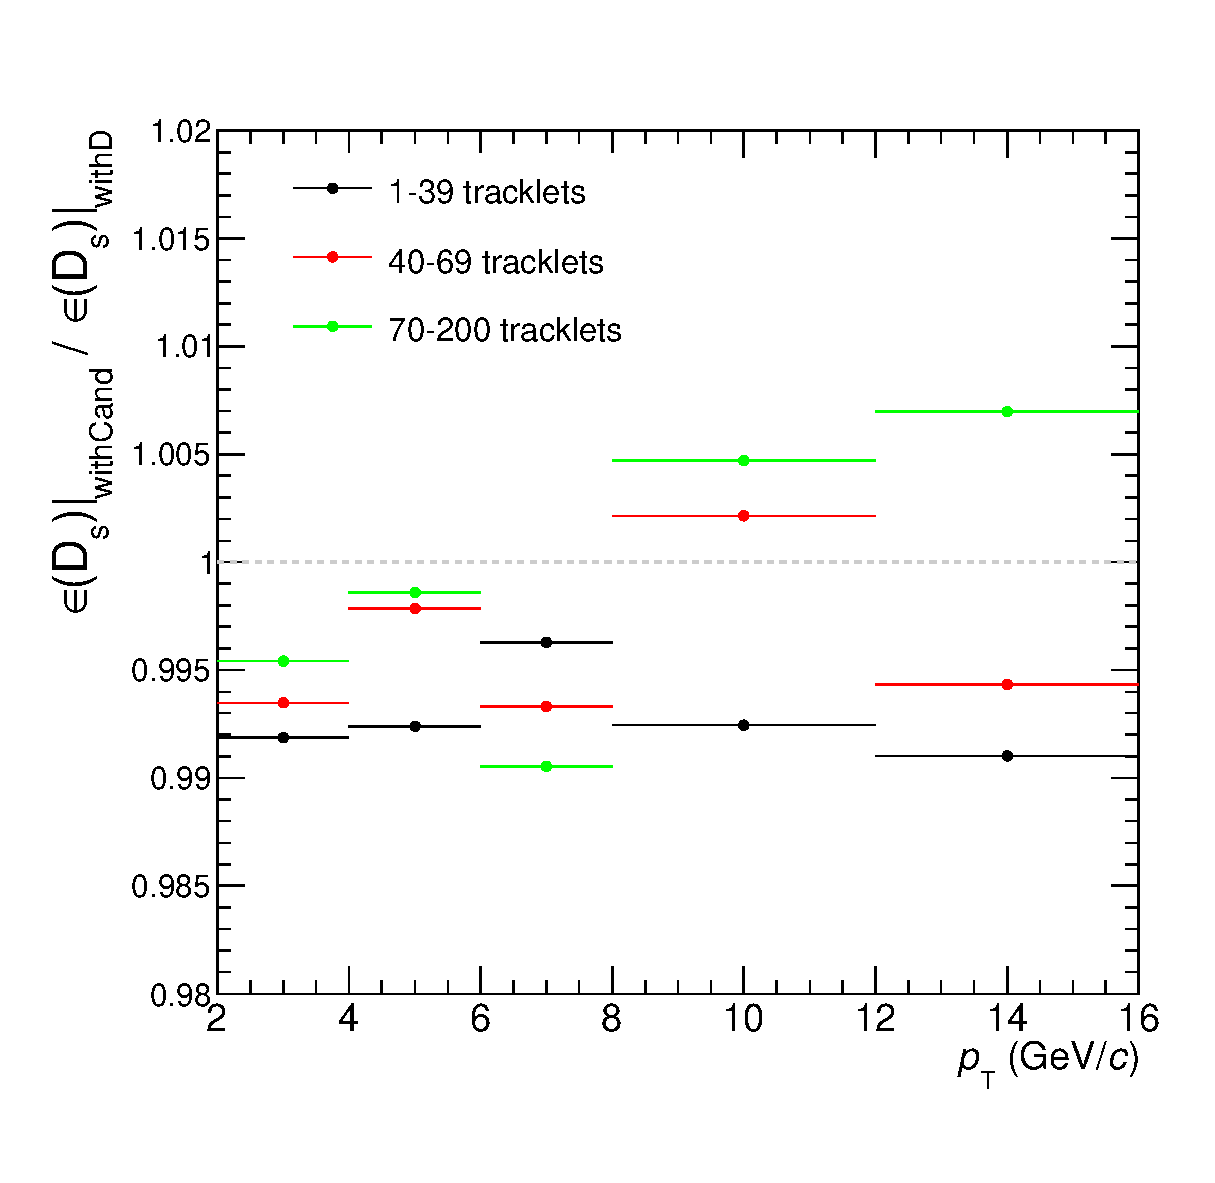
\includegraphics[width=.49\textwidth]{FigCap6/SystOnDWeightsWithCandVsWithD_Dsonly.eps}
 \caption{Ratio between the efficiency obtained with these weights, compared to the default ones, for $\Dplus$ (right) and $\Ds$ (left).}
 \label{fig:DsDplusVsMult_SystEffWeights}
\end{figure}


In the $\Ds/\Dplus$ yield ratios, the following sources of systematic 
uncertainties were considered as uncorrelated:
\begin{itemize}
\item raw-yield extraction;
\item selection efficiency;
\item PID selection efficiency;
\item generated D-meson $\pt$ shape (negligible);
\item hypothesis on $\RpPb^{feed-down}$ for the feed-down D meson subtraction;
\end{itemize}
while:
\begin{itemize}
\item efficiency correction with data-driven weights;
\item tracking efficiency;
\item variation of FONLL scales for the feed-down D meson subtraction;
\end{itemize} 
as fully correlated.


\begin{table}[h!]
\centering
\scalebox{0.9}{
\begin{tabular}{|l|c|c|c|c|c|}
\hline
 $\Ds$ syst. unc. (\%) & \multicolumn{5}{c|}{$\pt$ interval ($\GeV/c$)}\\
\hline
 $1 \leq \Ntrkl < 40$ & 2--4  & 4--6 & 6--8 & 8--12 & 12--16 \\
\hline
Yield extraction & 4 & 4 & 3 & 3 & 9\\
Selection efficiency  & 14   &   9   &     8	& 8	&7\\
PID efficiency &  2 & 2 & 2 & 2 & 2 \\
Tracking efficiency & 4 & 4 & 4 & 4 & 4 \\
MC $\pt$-shape & negl & negl & negl & negl & negl \\
Feed-down  &	$^{+3}_{-4}$	& $^{+3}_{-4}$ & $^{+3}_{-4}$ & $^{+3}_{-4}$	&$^{+5}_{-5}$\\
Multiplicity weights & 1 &  1 &  1 &  1 &  1 \\
\hline
 $40 \leq \Ntrkl < 70$ & 2--4  & 4--6 & 6--8 & 8--12 & 12--16 \\
\hline
Yield extraction & 3 & 3 & 4 & 5 & 12\\
Selection efficiency & 14 & 9 & 8	& 8	&7\\
PID efficiency&  2 & 2 & 2 & 2 & 2 \\
Tracking efficiency& 4 & 4 & 4 & 4 & 4 \\
MC $\pt$-shape & negl & negl & negl & negl & negl \\
Feed-down  &	$^{+3}_{-4}$	& $^{+3}_{-4}$ & $^{+3}_{-4}$ & $^{+3}_{-4}$	&$^{+5}_{-5}$\\
Multiplicity weights & 1 &  1 &  1 &  1 &  1 \\
\hline
 $70 \leq \Ntrkl < 200$ & 2--3  & 4--6 & 6--8 & 8--12 & 12--16 \\
\hline
Yield extraction   & 4 & 4 & 4 & 4 & 10\\
Selection efficiency & 14 & 9 & 8	& 8	&7\\
PID efficiency&  2 & 2 & 2 & 2 & 2 \\
Tracking efficiency& 4 & 4 & 4 & 4 & 4 \\
MC $\pt$-shape & negl & negl & negl & negl & negl \\
Feed-down  &	$^{+3}_{-4}$	& $^{+3}_{-4}$ & $^{+3}_{-4}$ & $^{+3}_{-4}$	&$^{+5}_{-5}$\\
Multiplicity weights & 1 &  1 &  1 &  1 &  1 \\
\hline
\end{tabular}}
\caption{Systematic uncertainties on $\Ds$ for the $\Ds/\Dplus$ versus multiplicity measurement.}
\label{tab:DsVsMult_syst}
\end{table}

\section {Conversion of $\Ntrkl$ to primary charged particles}
\label{sec:NtrklToNch}
The conversion of the number of tracklets to the average multiplicity of primary charged particles ($\Nch$) 
was performed using a minimum-bias Monte Carlo production using EPOS generator~\ref{Drescher:2000ha}. 
The distribution of the reconstructed $\Ntrkl$ as a function of the number of
$\Nch$ in the simulation was considered for this purpose, and it is shown in Fig.~\ref{fig:NtrklVsNch} (left).
The $z-$axis of the 2D correlation was re-weighted with data-driven $\Ntrkl$ weights, to model the tracklet
distribution in the minimum-bias production to that in data. 
The mean profile of distribution was fitted with a linear function, and their ratio
is presented in Fig.~\ref{fig:NtrklVsNch}. The correlation between $\Ntrkl$ and $\Nch$ 
was treated as linear to extract the correction factor from tracklets to charged particles,
and further checks to test the non-linear correlation in particular for low and high values of
$\Nch$ were included in the systematic uncertainties.
The average value of charged particles in each multiplicity interval
was calculated from the average $\averNtrkl$ value in each class 
times the conversion factor from the linear fit.
These values, shown in Fig.~\ref{fig:Nch}, were then divided by the 
width of the considered $\eta$ range, $\Delta \eta =$ 2, 
to obtain $\langle {\rm d} \Nch/{\rm d}  \eta \rangle |_{|\eta|<0.5}$.\\



To estimate the systematic uncertainties on the evaluation of the average 
$\Nch$ values in the considered $\Ntrkl$ intervals, three different tests have been performed.
\begin{enumerate}
\item The conversion from $\Ntrkl$ to $\Nch$ was repeated with different MC generators. The correlation
between $\Ntrkl$ to $\Nch$ can in fact be sensitive to the primary and secondary particle cocktail used in the event generator.
In particular, minimum-bias Monte Carlo 
productions with EPOS and DPMJET generators were compared.
The comparison of the average $\Nch$ obtained from the two MC productions
is presented in Fig.~\ref{fig:NchVsMCgenerator}.
\item The conversion from $\Ntrkl$ to $\Nch$ was repeated changing the 
assumption on linearity of the correlation. This was done to test deviations from 
the linear correlation between $\Ntrkl$ and $\Nch$, which is  
observed in particular at low and high multiplicity, as displayed in the right panel of Fig.~\ref{fig:NtrklVsNch}.  
The average $\Nch$ was extracted by: (i) fitting the 2D histogram with a second-order polynomial 
function; (ii) considering the average $\Nch$ values in the intervals corresponding to the $\Ntrkl$ 
classes considered in the analysis.
In Fig.~\ref{fig:NchVsCorrHypo} the comparison of the average $\Nch$ values
obtained with the three different methods (linear fit, parabolic fit and average of the $\Nch$ distributions) is shown.
\item The conversion from $\Ntrkl$ to $\Nch$ was repeated: (i) without the data-driven 
$\Ntrkl$ weights and (ii) applying the $\Ntrkl$ weights obtained considering all 
the events that pass the physics selection, with no any requirement to contain 
$\Dzero$ candidates. The comparison of $\Nch$ values from this test is shown in Fig.~\ref{fig:NchVsNtrklWithWOweights}.
\end{enumerate}
The three sources of uncertainties were considered as 
uncorrelated, therefore summed in quadrature. The final values for $\averNch$ in $|\eta|<1$ 
and the associated systematic uncertainties are shown in 
Fig.~\ref{fig:Nch}.

\begin{figure}[h]
\centering
 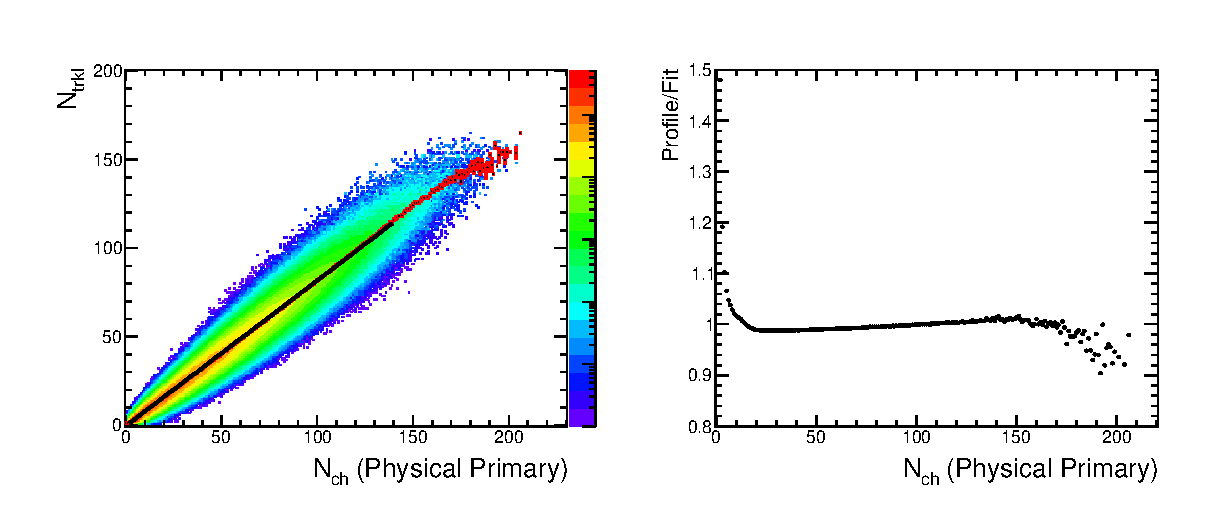
\includegraphics[width=1.\textwidth]{FigCap6/NtrklVsNchPhysPrimWithNtrklsReweight17f2a.eps}
 \caption{$\Ntrkl$ vs $\Nch$ distribution obtained for the 17f2a minimum bias production.}
 \label{fig:NtrklVsNch}
\end{figure}

\begin{figure}[h]
\centering
 \includegraphics[width=1.\textwidth]{FigCap6/NtrklNchDistrWithNtrklsReweight_17f2a.png}
 \caption{$\Ntrkl$ vs $\Nch$ distribution obtained for the 17f2a minimum bias production.}
 \label{fig:NtrklVsNch}
\end{figure}

\begin{figure}[h]
\centering
 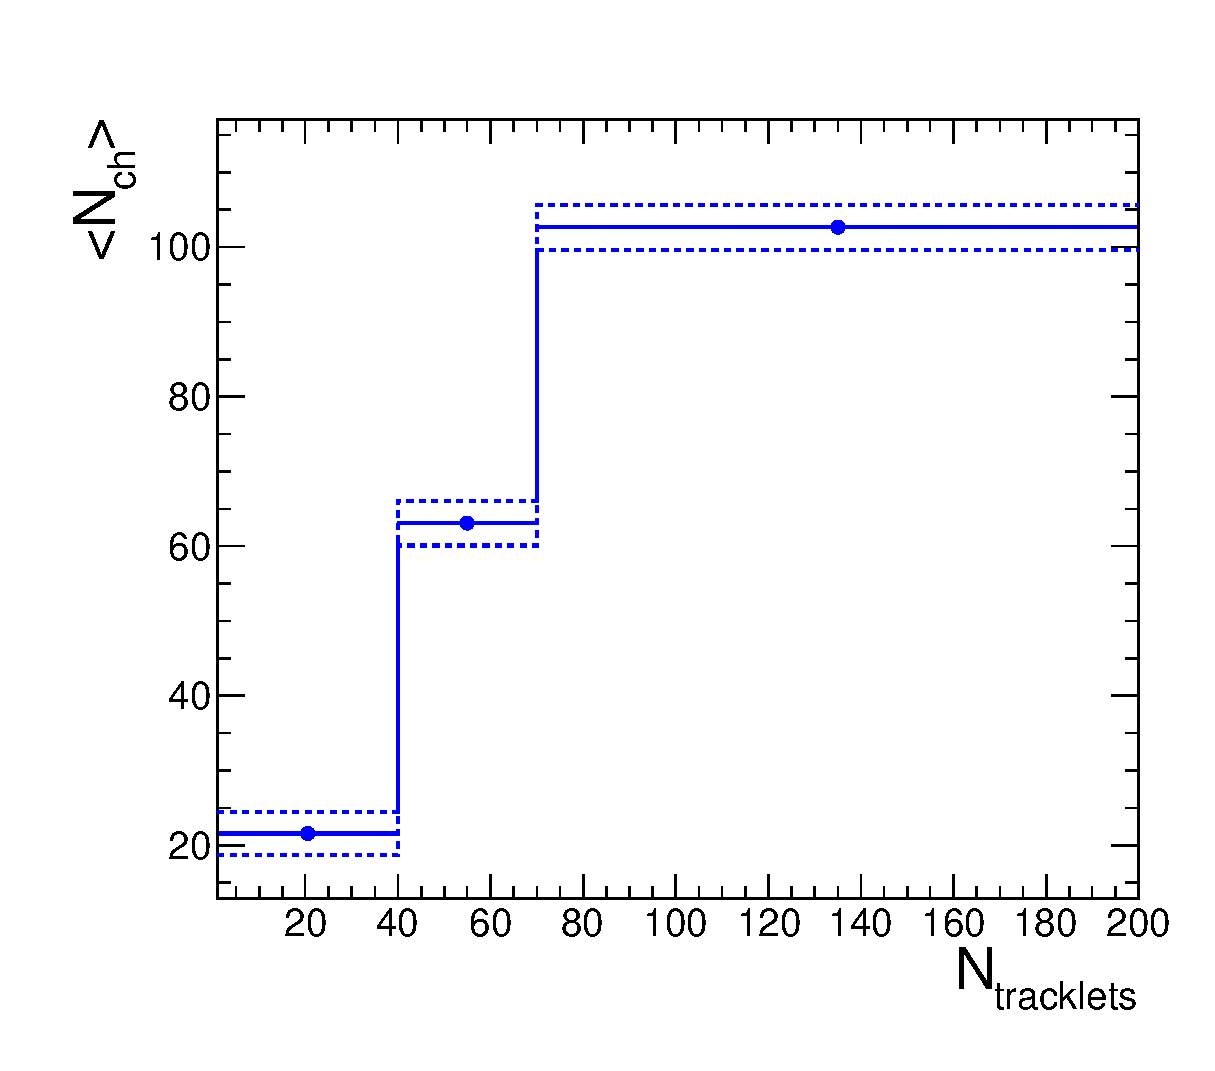
\includegraphics[width=.55\textwidth]{FigCap6/AverNchAndTotalSystUnc.eps}
 \caption{Average $\Nch$ values in the considered multiplicity classes, in the region $|\eta |< 1$. The lower and higher dashed lines represent the systematic uncertianties.}
 \label{fig:Nch}
\end{figure}

\begin{figure}[htpb]
\centering
 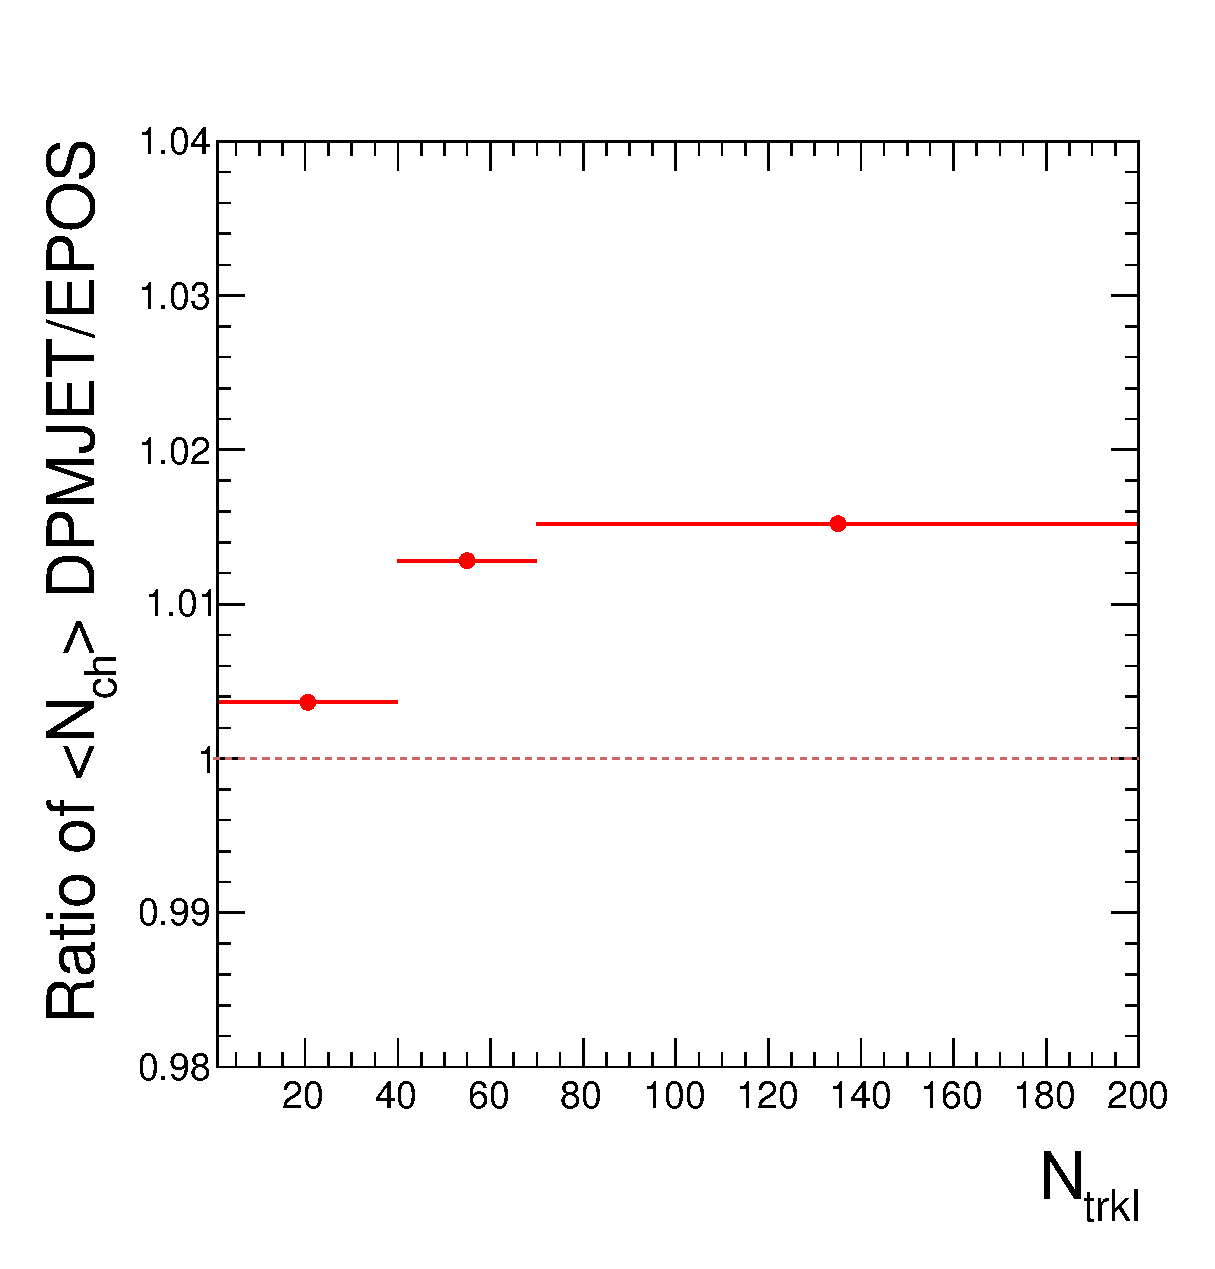
\includegraphics[width=.49\textwidth]{FigCap6/comparisonNtrkl_17f2b_17d2a_17f2a_onlySyst.eps}
 \caption{Left: Average $\Nch$ and $\Ntrkl$ values in the considered multiplicity classes, in the region $|\eta |< 1$, obtained from different MC productions. Right: ratio with respect to the default one (LHC172fa).}
 \label{fig:NchVsMCgenerator}
 \end{figure}


\begin{figure}[htpb]
\centering
 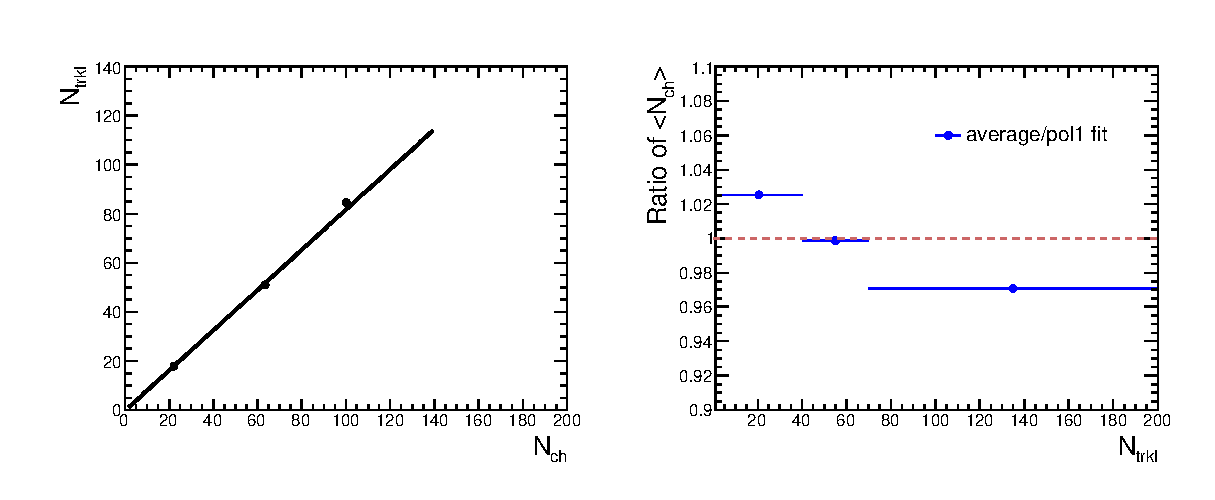
\includegraphics[width=1\textwidth]{FigCap6/NchSystematics_linFit_WithNtrklsReweight_17f2a.eps}
 \caption{Comparison of the average $\Nch$ obtained with the three different methods (linear fit, parabolic fit and mean of the $\Nch$ distribution).}
 \label{fig:NchVsCorrHypo}
 \end{figure}


\begin{figure}[htpb]
\centering
 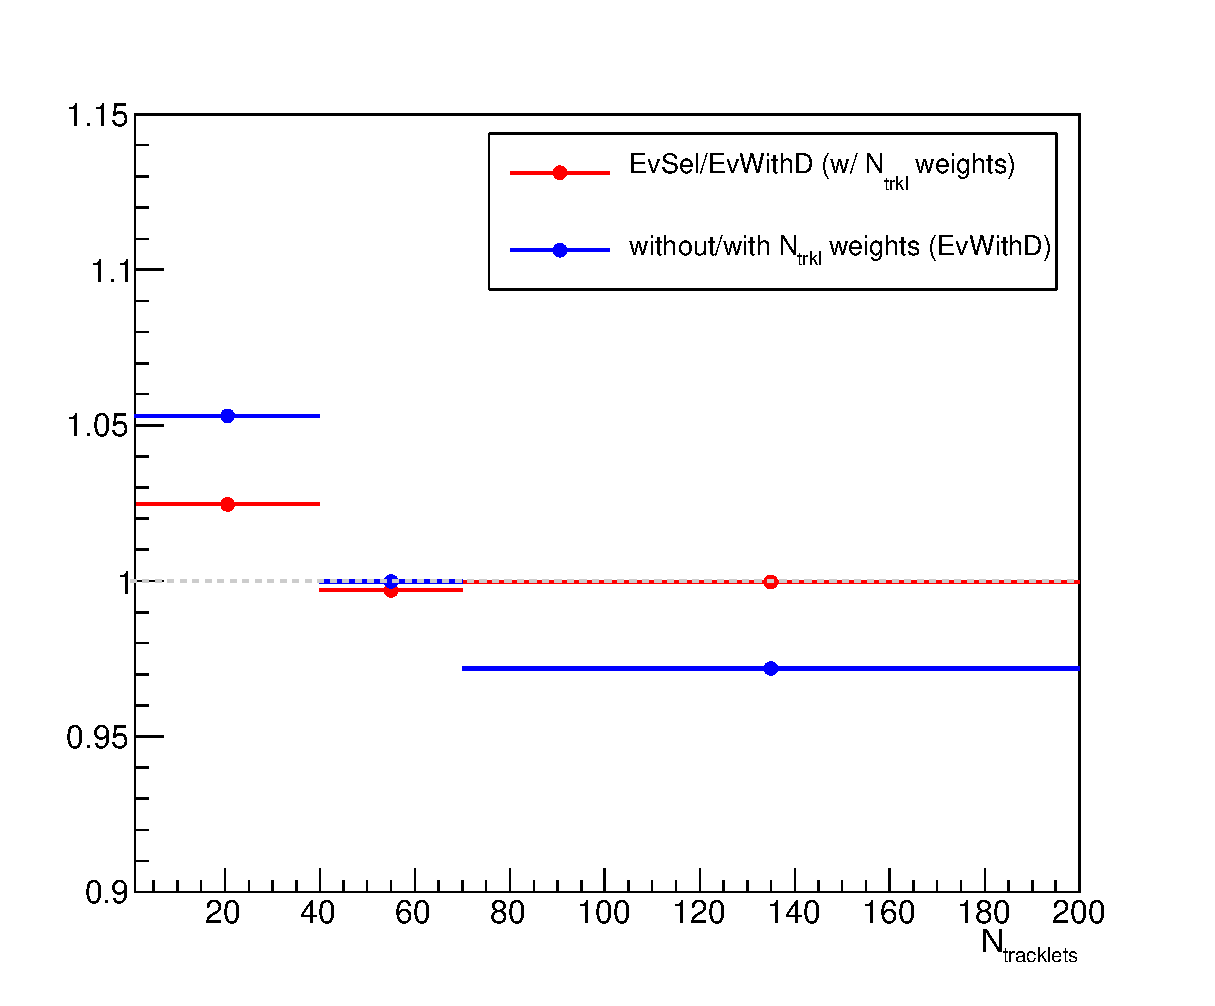
\includegraphics[width=.7\textwidth]{FigCap6/NchSystematics_NtrklWeights_17f2a.eps}
 \caption{Comparison of the average $\Nch$ obtained with and without data-driven $\Ntrkl$ weights.}
 \label{fig:NchVsNtrklWithWOweights}
 \end{figure}


\section{Results}
\label{sec:results}
The ratios of $\Ds/\Dplus$-meson yields are shown in Fig.~\ref{fig:DsDplusRatios} as a function of
the average number of primary charged particles per unity of pseudo-rapidity, 
in five $\pt$ intervals from 2 to 16 $\Gevc$.
The already measured ratios in pp collisions at $\sqrt{s}=$7 TeV and 
in Pb-Pb collisions at $\sqrt{s_{\rm NN}}=$ 5.02 TeV
(for the 0-10\%, 30-50\% and 60-100\% centrality classes, in the 
$\pt$ intervals where they are available) are also reported in the figure.
A hint of a non-flat trend in the interval 2 $< \pt < 8~\Gevc$ is observed, although 
the points are compatible within their uncertainties. The measured points were 
fitted with a linear function to quantify their slope, considering the statistical 
uncertainties only in the fit. The slopes from the linear fit on the pp, 
p-Pb and Pb-Pb points were found to be different from zero within 
1$\sigma$ of the parameter error between 2 $< \pt < 8 ~\Gevc$, 
and between 4 $< \pt < 8 ~\Gevc$ for the fit on pp and p-Pb measurements only (Fig.~\ref{fig:FitRatios}).
The precision of this measurement will be improved using the 
larger data samples of p-Pb collisions that will be collected during the LHC Run-3.



\begin{figure}[h!]
    \begin{center}
          \includegraphics[width=0.9\textwidth]{./FigCap6/DsOverDplusVsMult_pp_pPb_PbPb.pdf}
    \end{center}
    \caption{ $\Ds/\Dplus$-meson yield ratios as a function of the primary charged particles in $|\eta|<0.5$, in the different $\pt$ intervals from 2 to 16 $\Gevc$.}
    \label{fig:DsDplusRatios}
\end{figure}

\begin{figure}[h!]
    \begin{center}
          \includegraphics[width=0.9\textwidth]{./FigCap6/Fit_DsOverDplusVsMult_pp7TeV_pPb5TeV_PbPb5TeV.pdf}
    \end{center}
    \caption{Linear fit on $\Ds/\Dplus$ ratios as a function of the primary charged particles, in the different $\pt$ intervals from 2 to 16 $\Gevc$. The slope of the pol1 is reported in each pad, for the fits made only on the pp and p--Pb measurements or on
    all the pp, p--Pb and Pb--Pb points.}
    \label{fig:FitRatios}
\end{figure}





